\title{Math 239 Fall 2023 Tutorial Answers Week 9}

\date{2023 Nov. 16/17}
\maketitle

\begin{enumerate}
    \question{Planar or Not}     
        The graph on the left is planar:
        \begin{figure}[h]
        \centering
            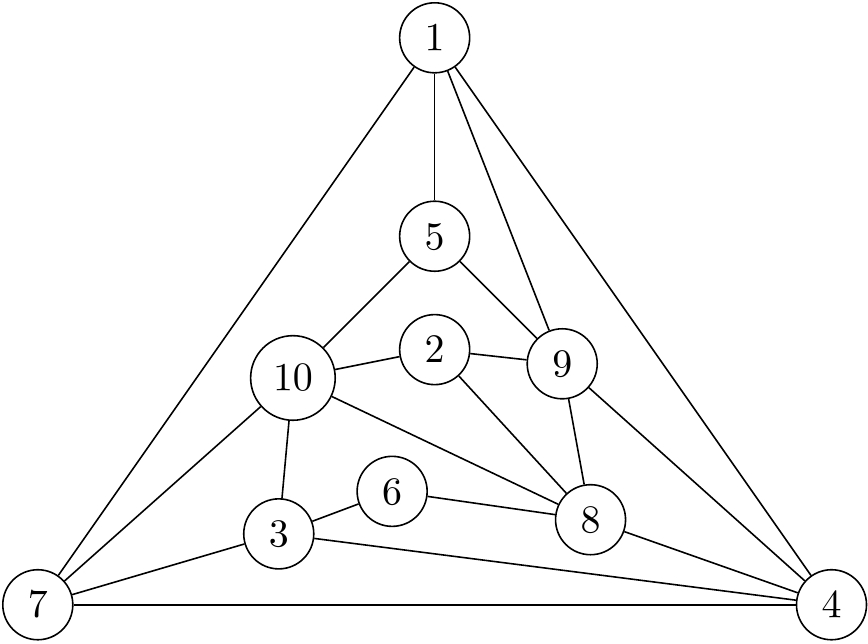
\includegraphics[width=.45\textwidth]{planar_soln.png}
        \end{figure}\\
        The graph on the right contains a subdivision of $K_{5}$
        \begin{figure}[h]
        \centering
             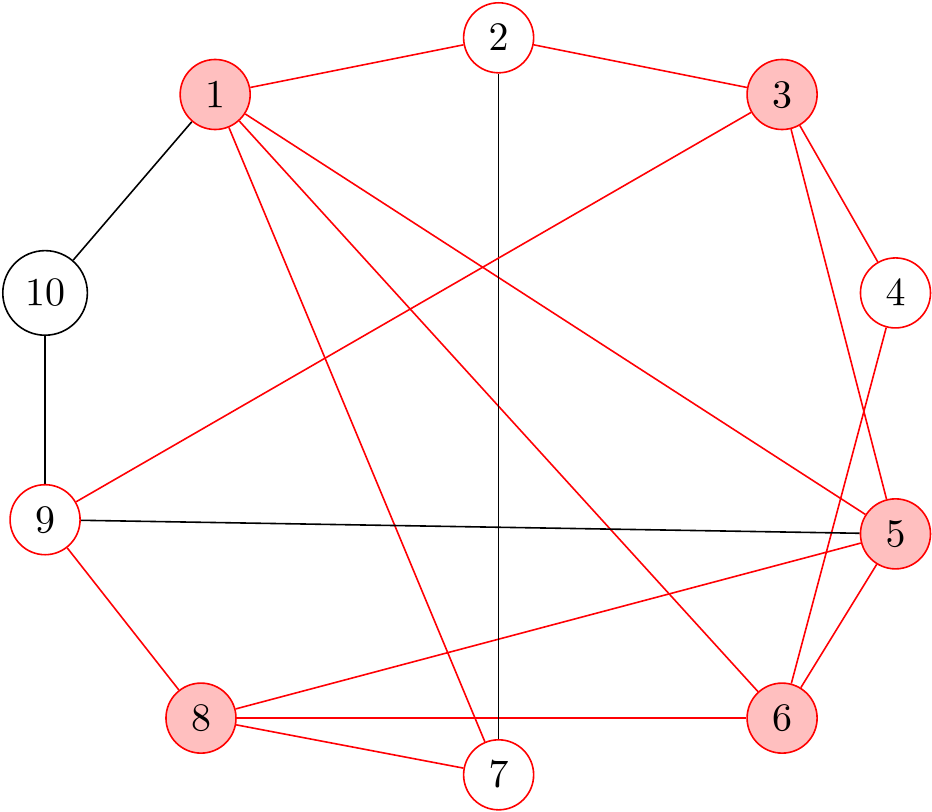
\includegraphics[width=.45\textwidth]{nonplanar_soln.png}\hfill
             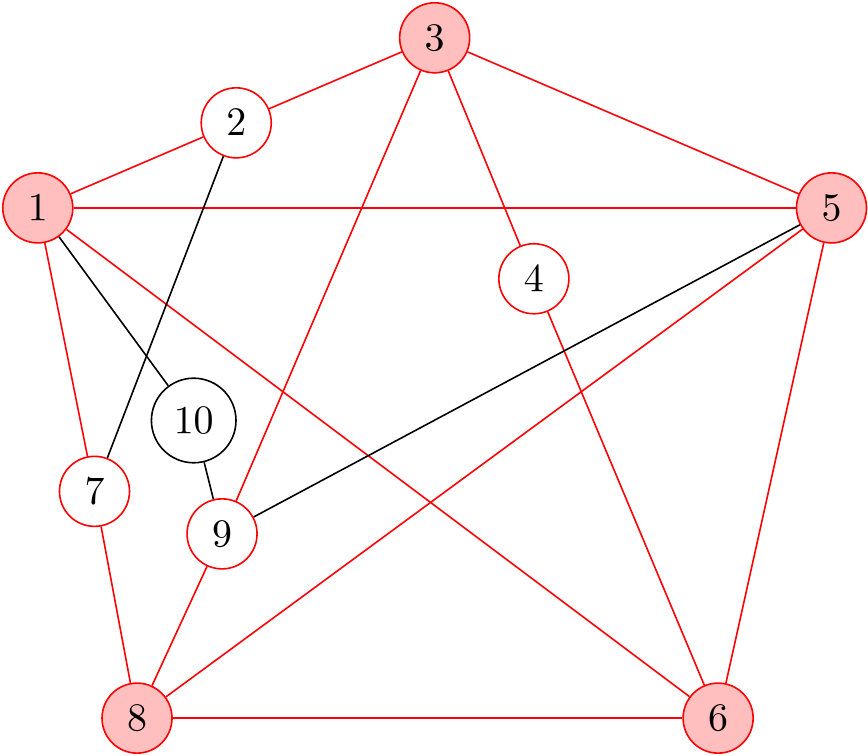
\includegraphics[width=.45\textwidth]{nonplanar_soln2.png}
        \end{figure}

   
    \question{Euler's Formula} 
    \begin{enumerate}
        \item Let $p_2, p_5, q$ and $s$ be the number of vertices of degree 2, number of vertices of degree 5, number of edges and faces in $G$. By Euler's formula, $p_2 + p_5 - q + s = 2$. By the two versions of handshake lemmas, $2p_2 + 5p_5 = 2q = 4s$. From the first equation, we obtain that $q = p_2 + p_5 + s - 2$. Substituting this to the other two equations, we obtain that
        \[2p_2 + 5p_5 = 2(p_2 + p_5 + s - 2) = 4s.\]

        From the first equation above, we obtain that $3p_5 = 2s -4$ and thus $2s = 3p_5 + 4$. Substituting this into the equation $2p_2 + 5p_5 = 4s$ we have $2p_2 + 5p_5 = 6p_5 + 8$. Hence $p_2 = (p_5 + 8)/2.$ Now, \[
        q = (2p_2 + 5p_5)/2 = \frac25 p_5 + \frac12 (p_5 + 8) = 3p_5 + 4.
        \]

        \item Given $p_5 = 4$, we immediately have $p_2 = (4+8)/2 = 6; q = 3\times 4 + 4 = 16; a = 3\times 4 /2 + 2 = 8$.
        
        Drawing
    \end{enumerate}

  
    \question{Complete Planar Tripartite Graphs} Consider $(a,b,c)$ and remember that $a \geq b \geq c$. Now consider $K_{a,b,c}$. Then deleting all the edges from part $B$ and part $C$ gives you $K_{a,b+c}$ as a subgraph. Then we can think about the various cases for $a$.
    \begin{enumerate}
        \item[$a \geq 3$:] Since $K_{a,b+c}$ is a subgraph then we must have that $b+c \leq 2$ (otherwise we have some $K_{3,3}$). Then the only possibility is $b=c=1$, which gives $K_{a,1,1}$ for all $a \geq 1$. Drawing this graph shows it is indeed planar.
        \item[$a \leq 2$:] the only possibilities are
        \begin{align*}
            (2,2,2), (2,2,1) , (2,1,1), (1,1,1).
        \end{align*}
        Then $K_{2,2,2}$ is planar from the following drawing. Then
        \begin{align*}
            K_{2,2,1}, K_{2,1,1},K_{1,1,1}
        \end{align*}
        are all planar as subgraphs of $K_{2,2,2}$.
    \end{enumerate}
    This gives exactly $K_{a,1,1}, K_{2,2,2}, K_{2,2,1}, K_{2,1,1},K_{1,1,1}$.

    \question{Partitioning Into Planar} Assume for contradiction that we can partition $K_n$ into $\lfloor \frac{n}{6} \rfloor$ planar subgraphs. Each subgraph has at most $n$ vertices, and we know from class that any planar graph on $n$ vertices can have at most $3n - 6$ edges. So in our partitioned graph, we'll have at most $\lfloor \frac{n}{6} \rfloor (3n - 6) \le \frac{n}{6} (3n - 6) = \frac{1}{2} (n^2 - 2n) = \frac{n(n-2)}{2}$. But our complete graph $K_n$ has $\frac{n(n-1)}{2}$ edges, which is more than $\frac{n(n-2)}{2}$. Therefore, we can't partition $K_n$ into  $\lfloor \frac{n}{6} \rfloor$ planar subgraphs.
\end{enumerate}